\documentclass[tikz]{standalone}
\usepackage{amssymb,dsfont}
\usepackage{color}
\usetikzlibrary{arrows}
% Sets
\newcommand{\CC}{\mathbb{C}}        % Complex numbers
\newcommand{\NN}{\mathbb{N}}        % Natural numbers
\newcommand{\RR}{\mathbb{R}}        % Real numbers
\newcommand{\ZZ}{\mathbb{Z}}        % Relative integers
% Groups
\newcommand{\SO}{\mathrm{SO}}       % Special orthogonal group
\newcommand{\OO}{\mathrm{O}}        % Orthogonal group
\newcommand{\SU}{\mathrm{SU}}       % Special unitary group
\newcommand{\1}{\mathds{1}}		    % trivial group
\newcommand{\DD}{\mathbb{D}}        % Dihedral group
\newcommand{\octa}{\mathbb{O}}      % Cubic (octahedral) group
\newcommand{\ico}{\mathbb{I}}       % Icosahedral group
\newcommand{\tetra}{\mathbb{T}}     % tetrahedral group
\begin{document}
	
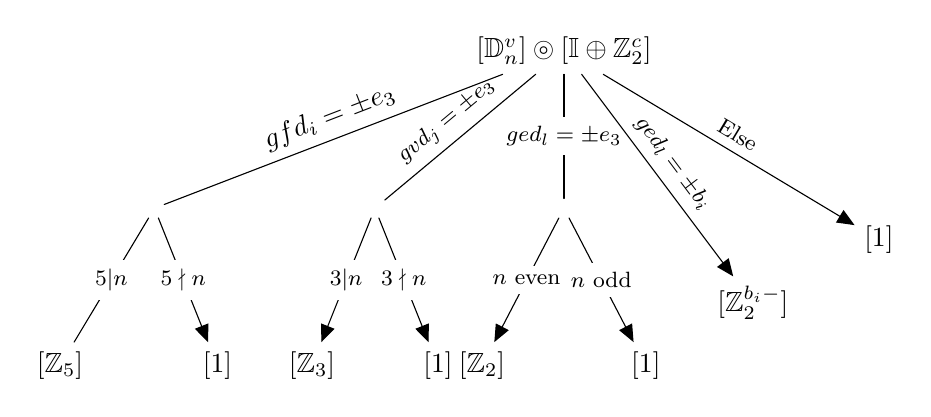
\begin{tikzpicture}[scale=0.8,line cap=round,line join=round,>=triangle 45,x=1.0cm,y=1.0cm]
  \node (root) at (0,0) {$[\DD_n^v]\circledcirc [\ico\oplus \ZZ_2^c]$};

  \node (Bas1) at (-6.5,-2.5) {};
  \node (Bas2) at (-3,-2.5)   {};
  \node (Bas3) at (0,-2.5)   {};
  \node (Bas4) at (3,-4) {$[\ZZ_2^{b_i-}]$};
  \node (Bas5) at (5,-3) {$[\1]$};
  \draw (root) -- (Bas1) node [midway,above,sloped] {{ $gfd_i=\pm e_3$ }};
  \draw (root) -- (Bas2) node [midway,above,sloped] {{\footnotesize  $gvd_j=\pm e_3$}};
  \draw (root) -- (Bas3) node [midway,fill=white] {{\footnotesize  $ged_l=\pm e_3$}};
  \draw[->] (root) -- (Bas4) node [midway,above,sloped] {{\footnotesize  $ged_l=\pm b_i$}};
  \draw[->] (root) -- (Bas5) node [midway,above,sloped] {{\footnotesize  Else}};
  \node (Bas11) at (-6.5-1.5,-5) {$[\ZZ_5]$};
  \node (Bas12) at (-6.5+1,-5) {$[\1]$};
  \draw (Bas1) -- (Bas11) node [midway,fill=white] {{\footnotesize  $5|n$}};
  \draw[->] (Bas1) -- (Bas12) node [midway,fill=white] {{\footnotesize  $5\nmid n$}};
  \node (Bas21) at (-3-1,-5) {$[\ZZ_3]$};
  \node (Bas22) at (-3+1,-5)  {$[\1]$};
  \draw[->] (Bas2) -- (Bas21) node [midway,fill=white] {{\footnotesize  $3|n$}};
  \draw[->] (Bas2) -- (Bas22) node [midway,fill=white] {{\footnotesize  $3\nmid n$}};
  \node (Bas31) at (-1.3,-5) {$[\ZZ_2]$};
  \node (Bas32) at (1.3,-5)  {$[\1]$};
  \draw[->] (Bas3) -- (Bas31) node [midway,fill=white] {{\footnotesize  $n$ even}};
  \draw[->] (Bas3) -- (Bas32) node [midway,fill=white] {{\footnotesize  $n$ odd}};
\end{tikzpicture}
% Further ’tikzpicture’ environments are possible which will create further pages.
\end{document} 